\documentclass[25pt, a0papper, portrait]{tikzposter}
\usepackage[utf8]{inputenc}
\usepackage{xcolor}
\usepackage{graphicx,mwe}
\usepackage{filecontents}% http://ctan.org/pkg/filecontents
\usepackage{lipsum}% http://ctan.org/pkg/lipsum
\usepackage{tikz}
\usepackage{multicol}
\usepackage{adjustbox}
\usepackage{color}
\usepackage[thinlines]{easytable}

\makeatletter
\def\TP@titlegraphictotitledistance{-9cm}
\settitle{ \centering \vbox{
		\@titlegraphic \\ [\TP@titlegraphictotitledistance] 
		\centering
		\color{titlefgcolor} {\bfseries \Huge \sc \@title \par}
		\vspace*{1em}
		{\huge \@author \par} \vspace*{1em} {\LARGE \@institute}
	}}
\makeatother
 
\title{TCPSnitch: Dissecting the Socket API Usage}
\author{\textbf{Gregory Vander Schueren}, Quentin De Coninck, Olivier Bonaventure \\ \texttt{gregory.vanderschueren@gmail.com} \\ \texttt{https://tcpsnitch.org}}
\date{\today}
\titlegraphic{
	
\includegraphics[width=0.06\textwidth]{figures/UCL}
    \hfill

\includegraphics[width=0.15\textwidth]{figures/tessares}
}

\institute{Université catholique de Louvain, Louvain-la-Neuve, Belgium}
 
\usepackage{blindtext}
\usepackage{comment}
\renewcommand*\familydefault{\sfdefault}
\usepackage[T1]{fontenc}
 
\usetheme{Desert}
\usenotestyle{Sticky}

\usepackage[backend=bibtex]{biblatex}
\addbibresource{biblio.bib,2011.bib}

\tikzposterlatexaffectionproofoff
\begin{document}
\maketitle

%{%<--------- Start scope
	\colorlet{notebgcolor}{yellow} %<---- change color
	%\block{BlocktitleB}{\lipsum[2]}
%}%<--------- End scope

% FIRST ROW
\begin{columns}
    \column{0.50}
    \block{New software: TCPSnitch}{
        \begin{itemize}
            \item Collects traces of the \textbf{interactions} between applications and the \textbf{TCP/IP stack}.
            \item \textbf{Tracks functions calls} on each socket with timestamp, parameters, return value, etc.
            \item Allows to \textbf{trace sequence of calls} and \textbf{detect patterns of interactions}.
            \item Runs on both \textbf{Linux and Android}.
            \item Comes with a \textbf{graphical interface} to visualize the traces: TCPSnitch.org.
            \item Leverages \texttt{LD\_PRELOAD} to intercept function calls.
            \item \textbf{TCPSnitch runs} the specified \textbf{command until it exits} like \texttt{tcpdump}.

        \end{itemize}
        \vspace{0.8cm}
        \begin{tikzfigure}
            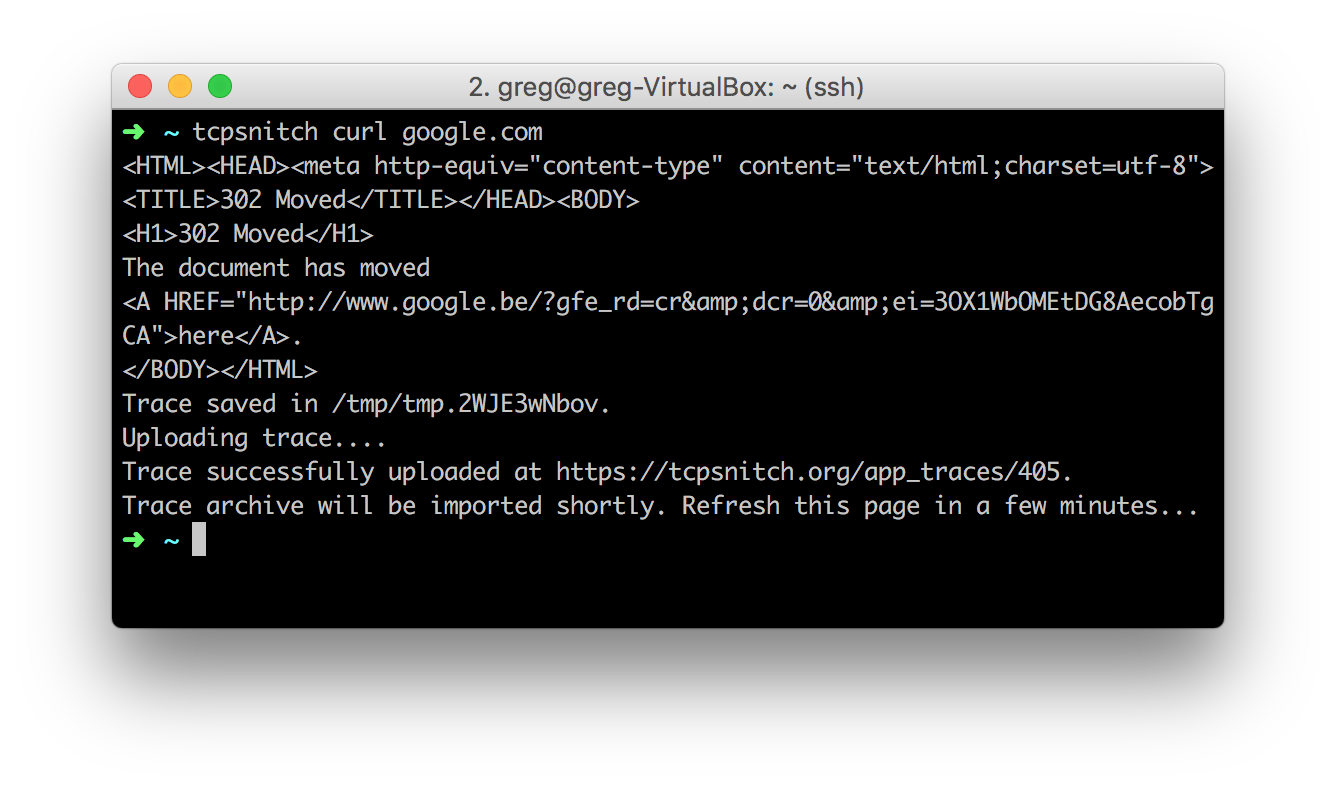
\includegraphics[width=.4\textwidth]{figures/tcpsnitch}
        \end{tikzfigure}
        \vspace{0.4cm}

        TCPSnitch is open-source: \url{https://github.com/GregoryVds/tcpsnitch}.
    }
    \column{0.50}
    \block{Public dataset: TCPSnitch.org}{
        \begin{itemize}
            \item TCPSnitch automatically \textbf{uploads traces to \url{https://tcpsnitch.org}}.
            \item Designed to \textbf{centralize and visualize the traces}.
            \item Contains \textbf{traces for} more than \textbf{130 applications} on Linux and Android.
            \item Dataset represents about \textbf{5 M function calls on 25 K sockets}.
            \item Provides \textbf{metrics and charts} at different levels of granularity: dataset, application, socket.
        \end{itemize}
        \vspace{0.8cm}
        \begin{tikzfigure}
            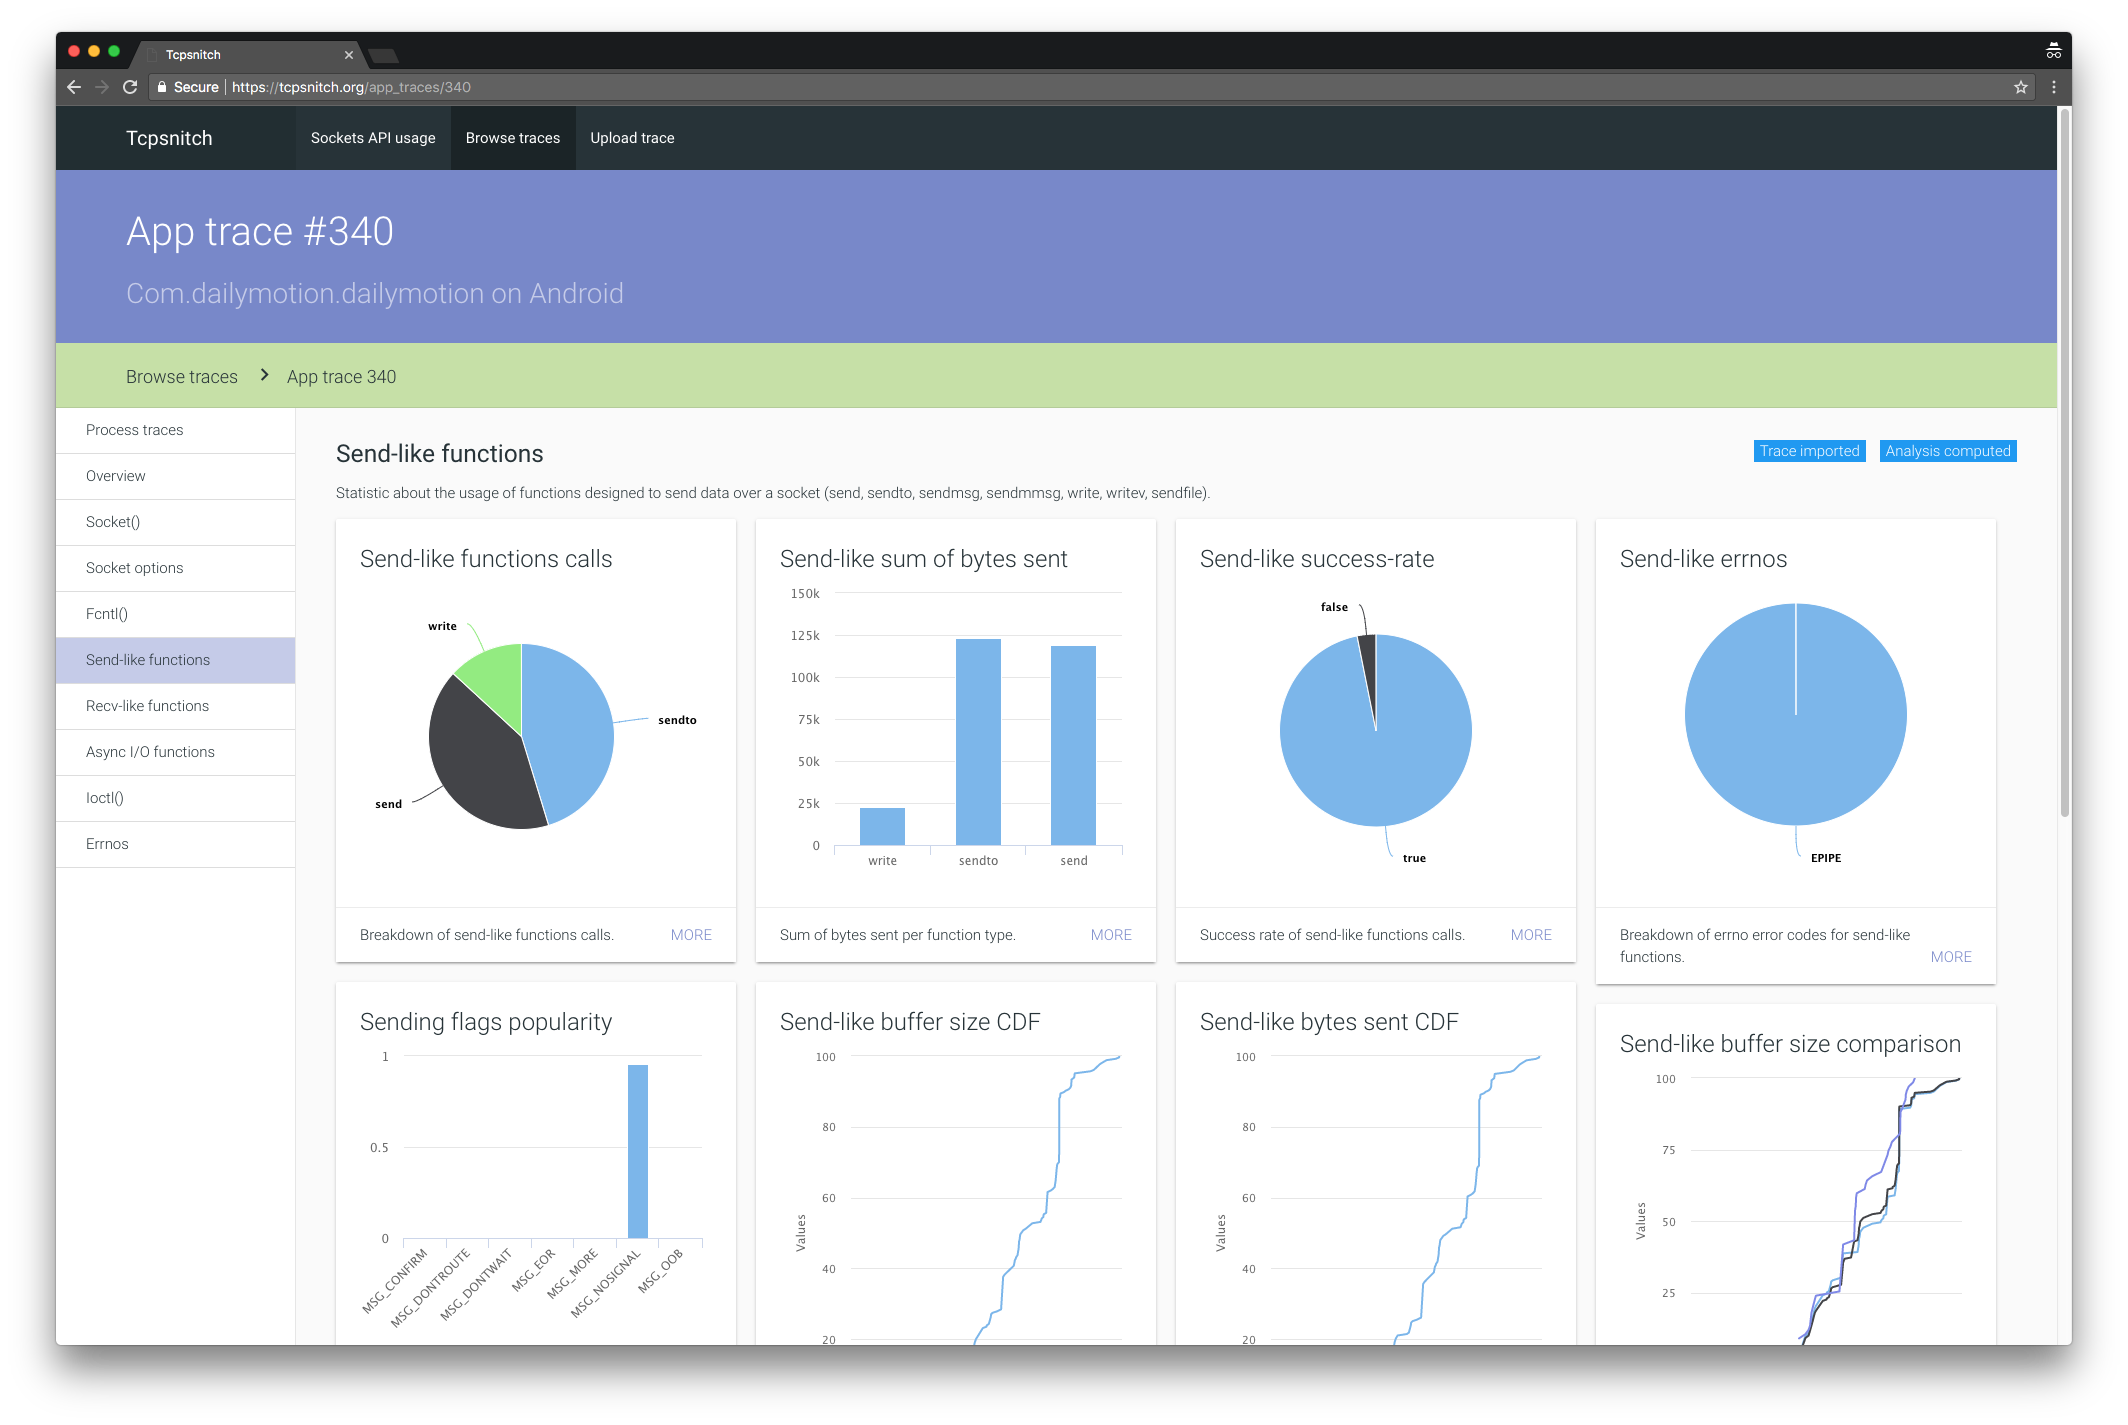
\includegraphics[width=.4\textwidth]{figures/org2}
        \end{tikzfigure}

        TCPSnitch.org is open-source: \url{https://github.com/GregoryVds/tcpsnitch_web}.
    }
\end{columns}



% THRID ROW
\begin{columns}
    \column{0.50}
    \block{API usage differs greatly on Linux and Android}{
        \begin{itemize}
            \item \textbf{Android application} appear more \textbf{homogeneous in} their \textbf{API usage}.
        \end{itemize}
        \begin{tikzfigure}
            \vspace{-1cm}
            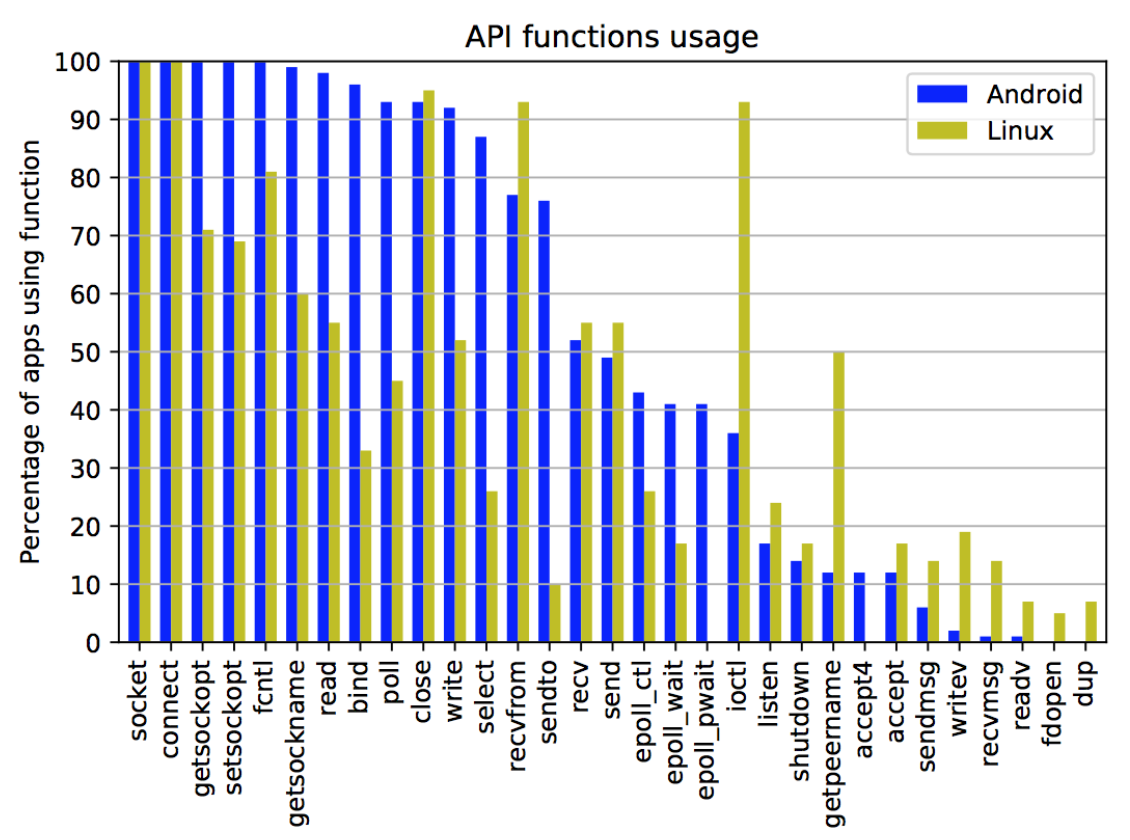
\includegraphics[width=0.40\textwidth]{charts/finding1}
        \end{tikzfigure}
    }
    \column{0.50}
    \block{API usage driven by high-level frameworks and libraries}{
    \begin{itemize}
        \item HTTP request over TLS yields \textbf{different API footprints with different libraries}.
        \item \textbf{No standard of doing things}, even for a simple HTTP request.
    \end{itemize}
    \vspace{1.5cm}
\begin{tikzfigure}
\renewcommand{\arraystretch}{2}
    \begin{tabular}{lllllll}
\hline
\textbf{Language}   & Ruby        & Python   & JavaScript        & Perl        & PHP\\ \hline
\textbf{Library}        & \texttt{Net:HTTP} & \texttt{urllib2}  & \texttt{https mod}  & \texttt{LWP::Simple} & \texttt{f\_g\_contents} \\ \hline
\textcolor{red}{\textbf{API calls}}  & \textcolor{red}{186}         & \textcolor{red}{353}    & \textcolor{red}{106}               & \textcolor{red}{465} &\textcolor{red}{920}\\ \hline
\textbf{Bytes recv} & 65~KB       & 175~KB   & 175~KB            & 178~KB      & 175~KB\\ \hline
\textbf{Main API call}  & \texttt{read()}      & \texttt{read()}   & \texttt{read()} & \texttt{read()}      & \texttt{fcntl()} \\ \hline
\textbf{Socket option}  & \texttt{TCP\_NODELAY} & \texttt{SO\_TYPE} & \texttt{SO\_ERROR} & \texttt{SO\_ERROR} & \texttt{SO\_ERROR}\\ \hline
\textcolor{red}{\textbf{Async I/O}}      & \textcolor{red}{\texttt{ppoll()}} &\textcolor{red}{N/A}      &\textcolor{red}{N/A} & \textcolor{red}{\texttt{select()}} & \textcolor{red}{\texttt{poll()}} \\ \hline
\end{tabular}
\end{tikzfigure}

        \vspace{2.8cm}
    }
\end{columns}


% FOURTH ROW
\begin{columns}
    \column{0.33}
    \block{Android: API functions usage}{
        \begin{itemize}
            \item Some \textbf{unexpected functions} are \textbf{widely used}.
        \end{itemize}
        \begin{tikzfigure}
            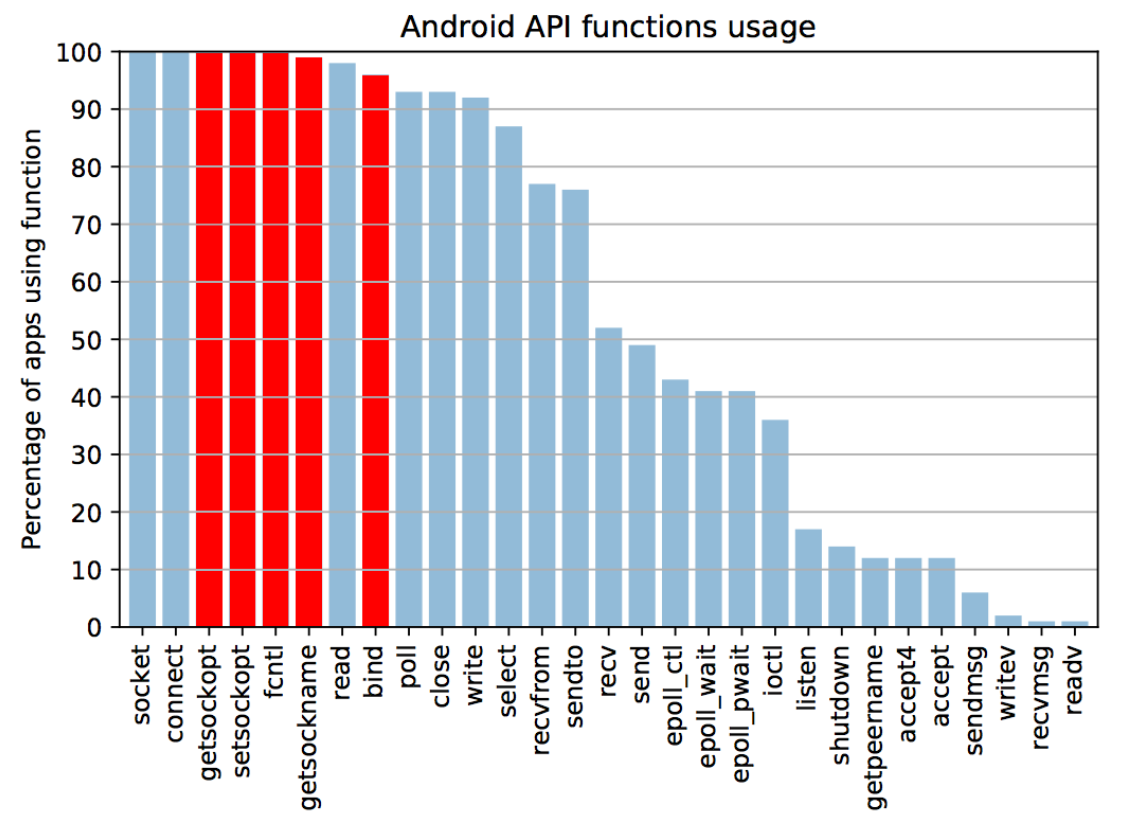
\includegraphics[width=0.25\textwidth]{charts/finding3}
        \end{tikzfigure}
        \vspace{0.1cm}
    }
    \column{0.33}
    \block{Android: UDP sockets usage} {
        \begin{itemize}
            \item \textbf{UDP sockets} are mainly \textbf{used to retrieve info about the network} configuration.
        \end{itemize}
        \begin{tikzfigure}
            \vspace{-0.6cm}
            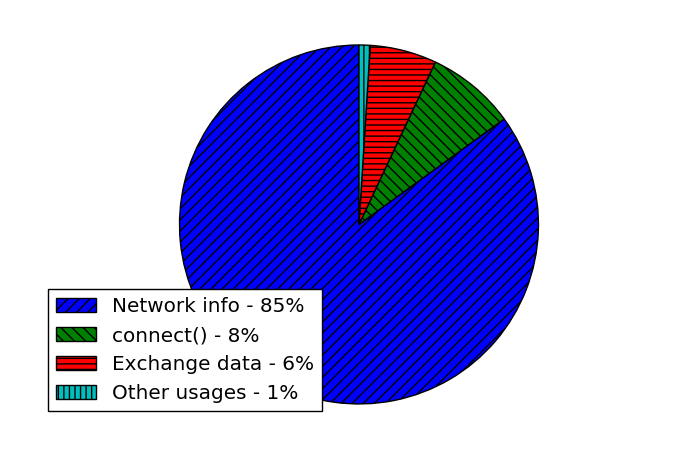
\includegraphics[width=0.28\textwidth]{charts/finding4}
        \end{tikzfigure}
    }
    \column{0.33}
    \block{Android: \texttt{TCP\_INFO} usage}{
        \begin{itemize}
            \item For some applications, the \textbf{number of \texttt{TCP\_INFO} calls} is a \textbf{linear function of the \texttt{recv()} calls}.
        \end{itemize}
        \begin{tikzfigure}
            \vspace{-1.1cm}
           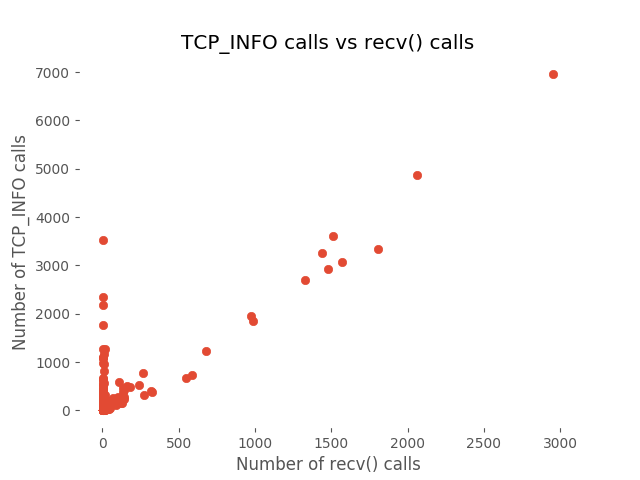
\includegraphics[width=0.25\textwidth]{charts/finding5}
        \end{tikzfigure}
%        \vspace{1cm}
    }
\end{columns}

\end{document}
